\documentclass[10pt,a4paper,oneside]{book}
%%% Para usar ecuaciones
\usepackage{amsmath}
\usepackage[spanish]{babel} % Corta palabras en espa~nol
%%% Para que quede en espaol
\usepackage[latin1]{inputenc}
\usepackage{graphicx}
\usepackage{afterpage}
%\usepackage{fullpage}
\usepackage{makeidx}
\usepackage{rotating}
\usepackage{verbatim}
\usepackage{alltt}
%Maneja colores
\usepackage{colortbl}
%%% Hyper vinculos
\usepackage{hyperref}
\hypersetup{colorlinks,%
citecolor=blue,%
filecolor=blue,%
linkcolor=blue,%
urlcolor=blue}
\begin{document}
	\title{EmotionBot: Architecture Description}
	%\author{Julian Mauricio Angel Fernandez}
	\maketitle
	\tableofcontents
	\newpage
	\begin{center}
		\begin{tabular}{|c|c|c|p{5.5 cm}|}
		\hline
		Version & Date &Author & Comments\\
		\hline
		 0.1&27/02/2014&Julian Angel & First draft of the system's design\\
		 \hline
		 0.2&23/05/2014&Julian Angel & Changes on the description design and addition on how works the decomposition of abstract action to simple action\\
		 \hline
		\end{tabular}
	\end{center}
	\newpage
	%%%%%%%%%%%%%%%%%%%%%%%%%
	\chapter{General View}
	The architecture presented in this chapter was created following the Belief, Desires and Intentions (BDI) approach, as could be seen in the Figure~\ref{fig:GeneralArchitecture}  !!WRITE WHY IT WAS CHOSEN THIS APPROACH. Additionally to the modules BDI, it was added the modules of action modulation and description. The description module is used to create information that it could be used by the robot as: the script, normal speed, etc.
\begin{figure}
	\centering
	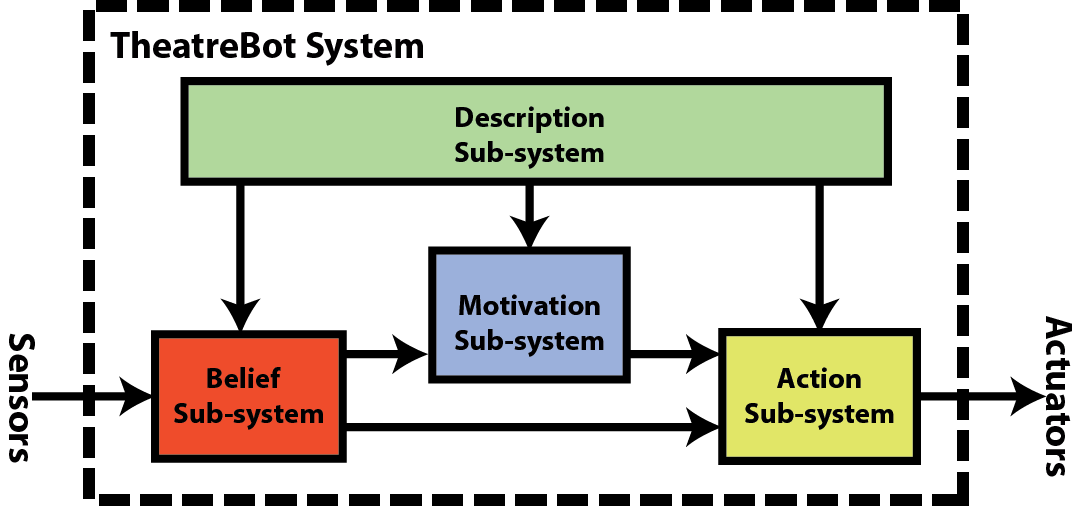
\includegraphics[width=1.0\textwidth]{./Images/Architecture/GeneralArchitecture.png} 
	\caption{General Architecture. The dash line shows the components that are in the system. The concepts of Desires and Intentions are included in the box Motivation.}
	\label{fig:GeneralArchitecture}
\end{figure}
Each of the modules are decomposed in sub-system that working as a whole could be used to accomplish the task. The final result could be seen in the Figure~\ref{fig:ArchitectureWithSubSystems}, where the module Action was divided in two: Action decision and Action modulation. Also was added the sub-module feature. Each of the modules in the architecture will be described in more detail though this chapter. 
\begin{figure}
	\centering
	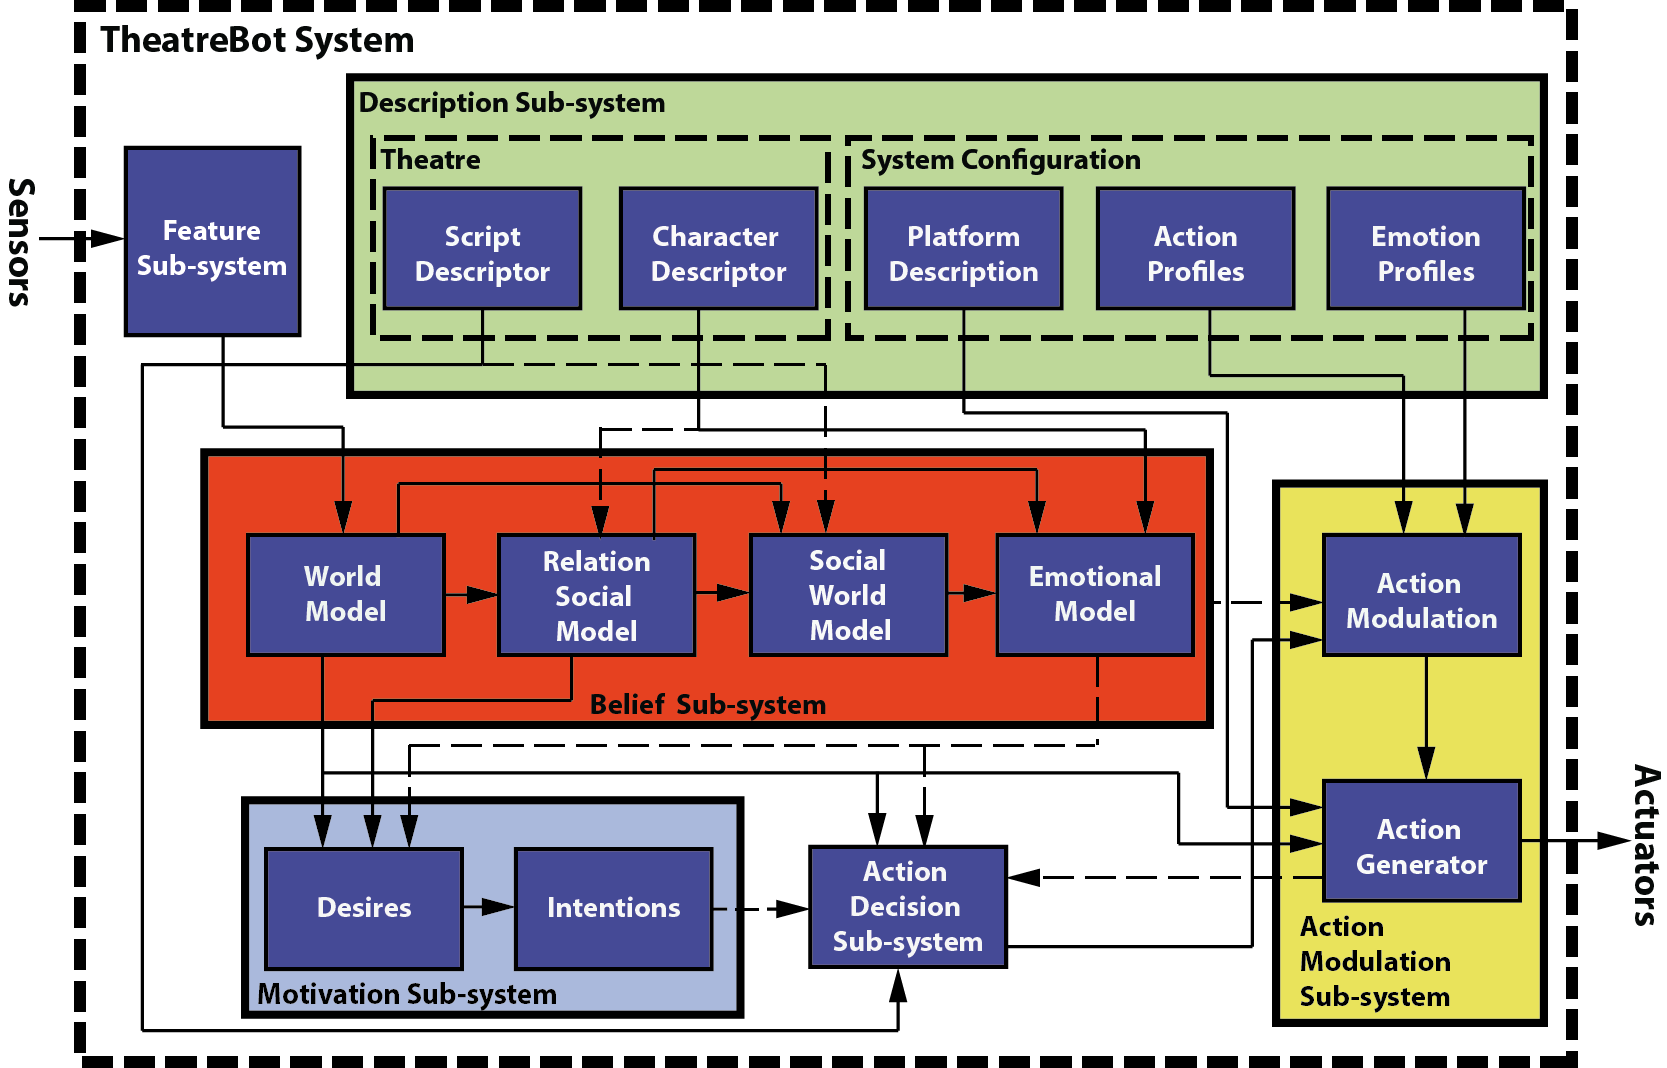
\includegraphics[width=1.0\textwidth]{./Images/Architecture/ArchitectureNew.png} 
	\caption{Architecture with the subsystems.}
	\label{fig:ArchitectureWithSubSystems}
\end{figure}
The whole action system is based on two main concepts: simple actions and abstract actions.
%%%%%%%%%%%%%%%%%%%%%%%%%
\subsection{Simple Action}
The simple actions are actions that have specialized modules that execute them. In order words they are already implemented and are platform dependent, thus it should be a different implementation of the action for the each platform that should be supported. In the first implementation, simple action should be follow the next characteristics:
\begin{itemize}
	\item Simple action controllers are not aware about other simple action controller. The synchronization is done through other module.
	\item Actions that are using the same actuators should be additive. For example the action move and oscillatemove are additive because oscillatemove is just going to introduce oscillation given an angle $theta$, thus the $theta$ could be modified by move. These actions two actions are controlled by the same controller, but its interface is different.
\end{itemize} 
At the moment the current actions are:
\begin{itemize}
	\item $Move(finalposition,trajectoryDescription)$ where finalPosition is the vector $<x,y,\theta>$ and velocity is a vector $<velocity\_x,velocity\_y,velocity\_\theta>$. The controller for this action should move the robot from its current position to the desire position. It is important to notice that the controller must also have as an input the world model in order to avoid obstacles. The trajectoryDescription is optional, thus if there is not given any information on this, the default values are used.
	\item $OscillateMove(velocity\theta,maximumAngle,trajectoryDescription)$ the oscillation movement just implies movement in the angular velocity, thus it is just change in the $\theta$ component, and $maximumAngel\in[\pi,-\pi)$
	\item $RotateTorso(angle,trajectoryDescription)$ moves the upper part of the waist, if there is one.
	\item $OscillateTorso(velocity,maximumAngle)$ which enable the oscillation of the upper part of the waist.
	\item $Grasp(object)$ try to grasp the desire object
	\item $RotateHead(angle\theta,angle\beta,angle\omega,velocity\theta,velocity\beta,velocity\omega)$
	\item $OscillateHead(angelID,velocity,angle)$ where\\ $angleID\in \lbrace angle\theta,angle\beta,angle\omega \rbrace$
	\item $RorateShoulder(IDShoulder,angle\theta,angle\beta,velocity\theta,velocity\beta)$
	\item $OscillateShoulder(IDShoulder,angleID,velocity,maximumAngle)$ where\\ $IDShoulder\in (\forall x| x=shoulder\bigwedge x\in robot)$
	\item $Speak(text)$ where $text$ is the argument that should be said by the robot
\end{itemize} 
%%%%%%%%%%%%%%%%%%%%%%%%%
\subsection{Abstract Actions}
Abstract actions are actions that could be composed by other abstract or simple actions. For the composition of these kind of actions could be used any kind of synchronization constrains and structure. For example, one abstract action could be composed by other two actions that are executed concurrently or in serially. Right now, the time constrains are not considered.\\
The abstract action $walk_speak$ which has three parameters: $position$, $trajectory_description$ and $phrase$. This actions is composed by two actions: the abstract action $walk$ and the simple action $speak$. Note that the abstract action $walk$ is also composed by two simple actions: $move_body$ and $move_shoulders$.\\
The parameters of the abstract actions are explicit attached to the parameters of the actions that composed it. However, in not all the cases the parameters are covered by the abstract actions, thus it should be given an explicit value during the implementation and give a modification through the description system.




	\section{Description}
The action description defines all the necessary information that are required to generate emotive action and personalize the system. This system is divided into parts: general, which described the information to generate the emotive actions. And Theatre, which describes the script and the current character that should be portrayed by the robot.
%%%%%%%%%%%%%%%%%%%%%%%%%%%%
\subsection{Simple Actions}
The description saved for the simple actions are values by default for parameters of each action. If there is not any value for a parameters, it would be used as NULL. These parameters are override each time that the desire action has an explicit value for the parameter.
%%%%%%%%%%%%%%%%%%%%%%%%%%%%
\subsection{Abstract Action}
The abstract actions' description gives default values 
%%%%%%%%%%%%%%%%%%%%%%%%%%%
\subsection{Action Profile}
The action profiles describes the simple abstract actions that people have created based on the simple actions that are available in the system. It does not include any preconditions 
%%%%%%%%%%%%%%%%%%%%%%%%%%%
\subsection{Emotion Profile}
Emotions profiles are based on the research done during the first year, where we come up with some basic features that enable the emotion projection. Each abstract action has is own emotional profile and it should be described in terms of simple actions. Example:
\begin{verbatim}
<emotion id="happiness">
    <simpleAction id="Move">
		<parameter id="velocity">fast</parameter>    
    </simpleAction>
    <simpleAction id="OscillateMove">
        <parameter id="velocity">fast</parameter>
        <parameter id="maximumAngel">small</parameter>
    </simpleAction>
    <simpleAction id="BalanceArms">
        <parameter id="maximumAngle">medium</parameter>    
    </simpleAction>
    <simpleAction id="OscillateTorso">
        <parameter id="velocity">-fast</parameter>
        <parameter id="maximumAngel">small</parameter>
    </simpleAction>
</emotion>
\end{verbatim}
%%%%%%%%%%%%%%%%%%%%%%%%%%%
\subsection{Script descriptor}
%%%%%%%%%%%%%%%%%%%%%%%%%%%
\subsection{Character descriptor}
	\section{Action Modulation}
The principal role of this sub-system is to convert abstract actions (e.g. walk, gaze, etc.) and the emotional state to actions that could be performed by the robotic platform that it has been using. These emotions actions are just commands to the platform, but the emotional part is added during the process due to adding new simple actions, changing the parameters of the simple actions, or both. This could be done thanks that each abstract action should be describe in terms of simple actions, which the system knows how to modify and perform. The main inputs of these module are:
\begin{itemize}
	\item Emotion profiles, which is the information in how to show an emotion in terms of simple actions.
	\item Action profiles, which describes the basic actions and the composition of the abstract actions in terms of the simple actions. This is not longer truth because getting the information from the file implies that should be possible to generate the code from these files.
	\item Emotional state is described by the tuple emotion and intensity. The first says the emotions that is going to convey the robot, and the second says how much is going to be evident the emotion. Still missing the part of the intensity.
	\item Abstract action, which could be a simple action to a any action described in terms of the simple actions supported by the system.	
	\item Platform descriptions gives the information about which simple actions could be performed by the current platform.
	\item World model.
\end{itemize} 
The outputs of this module are:
\begin{itemize}
	\item \textit{Electronic signals:} to control each driver that has the robot.
	\item \textit{Failure signal:} to inform the action decision sub-system that one of the actions could not be performed.
\end{itemize}
This sub-system is sub-divided into two blocks: actions modulation and action generation.
%%%%%%%%%%%%%%%%%%%%%%%%%
\subsection{Action Modulation}
This module gets the emotional state and the action(s) to generate emotive actions, which includes adding new actions and modifying parameters of the current. To do this module add new actions regarding the platform. The inputs to this module are:
\begin{itemize}
	\item Emotion profiles
	\item Action profiles
	\item Emotional state
	\item Abstract action
\end{itemize}
The outputs:
\begin{itemize}
	\item \textit{Emotional actions:} are the set of simple actions with modified parameters to show emotions.
\end{itemize}
As well this module is divided in modules with specific objectives, the division could be seen in Figure~\ref{fig:actionModulation}. The goal of each module is described below:
\begin{itemize}
	\item \textit{Action decrypt:} take the abstract actions and converted to simple actions.
	\item \textit{Action addition:} add the new actions needed to show the emotion.
	\item \textit{Action modification:} changes the parameters of all the actions.
\end{itemize}
\begin{figure}
	\centering
	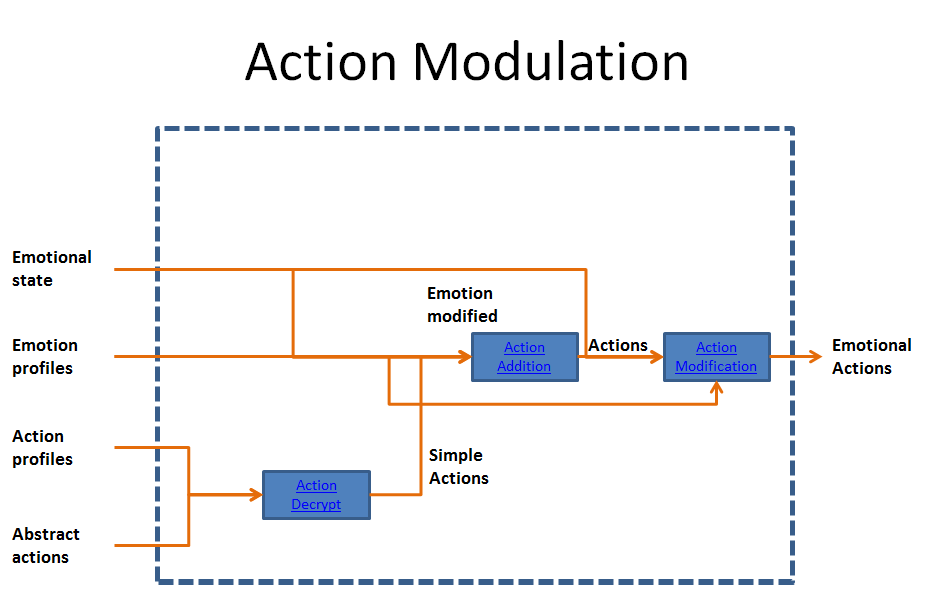
\includegraphics[width=1.0\textwidth]{./Images/Architecture/ActionModulation.png} 
	\caption{Modules of the action modulation sub-system}
	\label{fig:actionModulation}
\end{figure}
%%%%%%%%%%%%%%%%%%%%%%%%%
\subsection{Action Generation}
This module is in charge to decide which actions could be performed by the current platform, and execute and control each action that should be performed. The inputs of this module are:
\begin{itemize}
	\item Platform description
	\item Emotional actions
	\item World model
\end{itemize}
The outputs are:
\begin{itemize}
	\item Failure signal
	\item Signal controls
\end{itemize}
The task decomposition could be seen in Figure~\ref{fig:actionGeneration}. The goal of each sub-module are described below:
\begin{itemize}
	\item \textit{Action filter:} filters the possible actions that could be perform due the constrains of the platform, and it makes any necessary change to the action to be correct performed by the platform (e.g. Constrains of movement)
	\item \textit{Action controller:} decides which actions should be executed given the current actions that have performed by the robot. This module communicates with a specific module, which knows how to perform the action. This module knows which actions are executing and solve the problems of precedence and importance.
	\item \textit{Specific controllers:} are modules developed with the idea to execute an specific simple action.
\end{itemize}
\begin{figure}
	\centering
	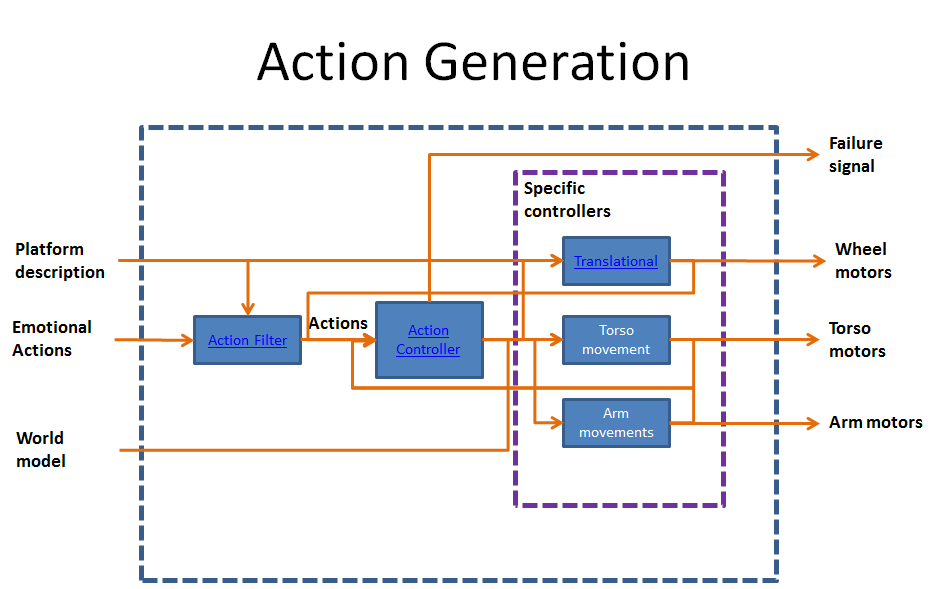
\includegraphics[width=1.0\textwidth]{./Images/Architecture/ActionGeneration.png} 
	\caption{Modules of the action generation}
	\label{fig:actionGeneration}
\end{figure}
	\section{Belief}
%%%%%%%%%%%%%%%%%%%%%
\subsection{Relational Social Model}
This module upgrades the relations with other people and roles, and the emotions that these produce to the character. The inputs of this module are:
\begin{itemize}
	\item World model
	\item Character descriptor, which gives the concrete information of the relation during a play. This allow focus in the other modules and test the system.
\end{itemize}
The output of this module is:
\begin{itemize}
	\item A list of people and roles that are in the current situation, and the emotions that these produce in the character.
\end{itemize}
%%%%%%%%%%%%%%%%%%%%%
\subsection{Social World Model}
This module is in charge to recognize the current social situation and determine other's emotional state. The inputs of this module are:
\begin{itemize}
	\item World model
	\item A list of people and roles that are in the current situation, which is used as a filter.
	\item Script descriptor, which gives information of the current situation and the emotional state of the other people present in the current scene.
\end{itemize}
The outputs are:
\begin{itemize}
	\item Social situation
	\item List of the people present in the environment and their respective emotional state
\end{itemize}
%%%%%%%%%%%%%%%%%%%%%
\subsection{Emotional Model}
This module calculates the current emotional state based on the people present, their emotional state, and the current situation.
%%%%%%%%%%%%%%%%%%%%%
\subsection{World Model}
	%%%%%%%%%%%%%%%%%%%%%%%%%%
	\chapter{Requirements}
		\begin{itemize}
		\item How to change the emotional state without changing the current action?
		\item How to change the action without the emotional state?
		\item How to handle when the emotional state changes and the action is the same?
		\item How to describe the script?
		\begin{itemize}
			\item How to handle the questions written above?
			\item Is it necessary to introduce time?
			\item How to add the coordination points?
			\begin{itemize}
				\item Levels of these points?
			\end{itemize}
		\end{itemize}
		\item Which is the best way to describe the abstract actions, emotions profiles, etc.?
		Possibilities:
		\begin{itemize}
			\item JSON
			\item XML
			\item YAML
		\end{itemize}
		Comparison:
		\begin{itemize}
			\item \href{https://www.udemy.com/blog/json-vs-xml/}{JSON vs XML}
			\item \href{http://www.json.org/xml.html}{JSON vs XML}
			\item \href{http://yaml.org/spec/1.2/spec.html#id2759572}{YAML}
		\end{itemize}
		\item How to implement the specific controllers in ROS?
		\begin{itemize}
			\item the controllers depend on the platform?
		\end{itemize}
	\end{itemize}
	%%%%%%%%%%%%%%%%%%%%%%%%%%
	\chapter{Description Design}
	%%%%%%%%%%%%%%%%%%%%%%%%%%
	\chapter{Action Modulation Design}
	%%%%%%%%%%%%%%%%%%%%%%%%%%
	\chapter{Implementation}
	\input{./Implementation/Implementation}
\end{document}